\documentclass{article}
\usepackage{iclr2016_conference,times}

\usepackage{float}
\usepackage{hyperref}
\usepackage{url}
\usepackage{amsmath,amssymb}
\usepackage{natbib}
\usepackage{wrapfig}
\usepackage{graphicx}
\usepackage{soul}

\bibliographystyle{abbrvnat}


\usepackage{caption}
\usepackage{subcaption}

\title{
	Mobile Computing (CS23400$/$1) \vspace{-4pt} \\
	{\Large Lab 2 - Report} \vspace{6pt} \\
	{\large Andrea F. Daniele $\hspace{2.2cm}$ Max X. Liu $\hspace{2.2cm}$ Noah A. Hirsch}
}

\begin{document}

\maketitle


\vspace{-1.2cm}

\section{Task}
\vspace{-.3cm}
The goal of this lab is to identify the location of a Wi-Fi device by analyzing Received Signal Strength (RSS) data recorded by a Wi-Fi receiver mounted on a moving car. For each RSS reading, we can estimate the distance from the car to the Wi-Fi device and thus create a circular locus of possible locations around the car. As we collect multiple RSS readings from the moving car, we can create multiple loci whose intersection locates the position of the Wi-Fi device. We must also overcome the RSS noise due to variable environments and signal reflection.

\section{Challenges}
\vspace{-.3cm}
The main challenge in this lab, as stated above, is mitigating RSS noise. To resolve this, our method chooses the single location in the workspace with the most locus intersections. Since we are collecting hundreds of RSS datapoints each second, the truthful datapoints will converge on the correct location, while the noisy datapoints will not converge on a single location as much to outweigh that correct answer. We believe this to be an appropriate solution, and it works for the test Wi-Fi devices of which we know the location.

Another challenge is that our car would often turn on its own, which would make it difficult to determine the car's position from its starting point, stopping point, and speed. This position is required to map the RSS locus to the workspace. Because of this, we were simply given the position of the car at each RSS reading, making this RSS mapping clear.

\section{Proposed Approach}
\vspace{-.3cm}
//TODO
\begin{wrapfigure}{r}{0.4\textwidth}
    \centering
    \vspace{-18pt}
    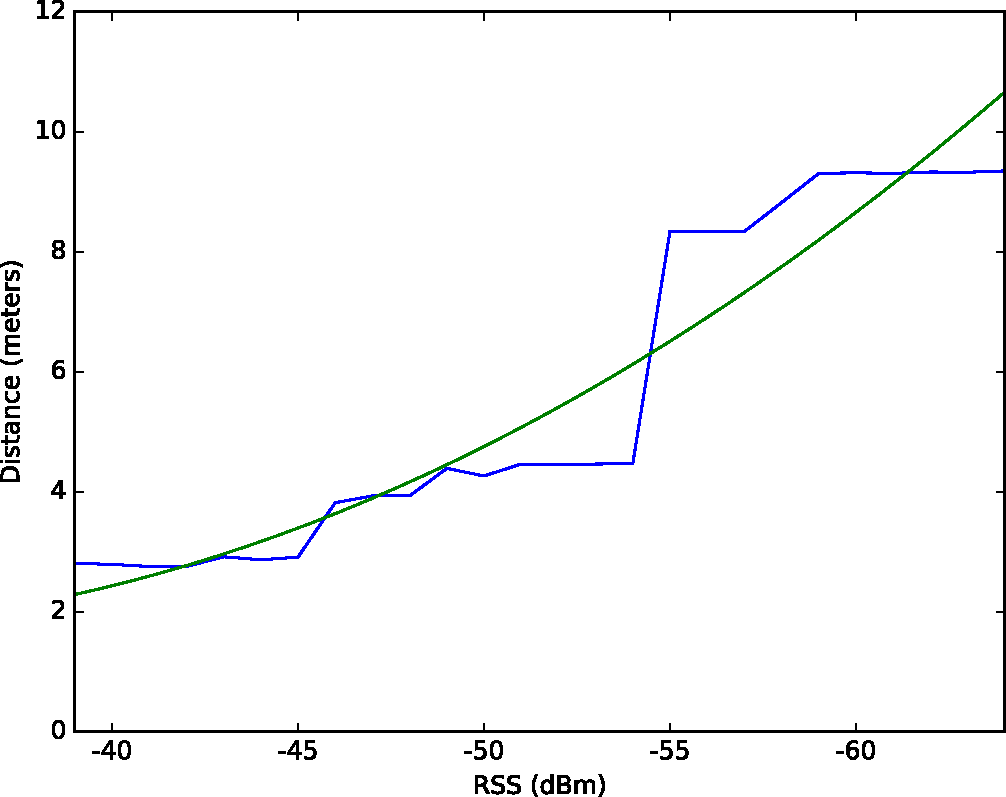
\includegraphics[width=\linewidth]{figures/rss_distance_plot.pdf}
    \caption{RSS-Distance relationship \label{fig:rss_distance_plot}}
\end{wrapfigure}


\section{Results}
\vspace{-.3cm}
We tested out approach on two WiFi camera for which we know the true location. Our
model predicted the location of the two cameras with $XX.XX$ and $XX.XX$ meters error.
Table~\ref{tab:results} shows the predicted location along with the prediction error for the
cameras for which the true location is unknown and the predicted locations for the hidden cameras.

\begin{center}
\begin{table}[h]
\centering
\begin{tabular}{ |c|c|c|c| } 
 \hline
 MAC & Predicted location (meters) & Ground-truth location (meters) & Error (meters) \\ 
 \hline
 8c:85:90:16:0a:a4 & $(7.25, 10.75)$ & $(6.8, 6.8)$ & $3.98$\\ 
 ac:9e:17:7d:31:e8 & $(X.x, Y.y)$ & $(0.87, 9.45)$ & $XX.XX$ \\ 
 d8:c4:6a:50:e3:b1 & $(X.x, Y.y)$ & $-$ & $-$ \\
 f8:cf:c5:97:e0:9e & $(X.x, Y.y)$ & $-$ & $-$ \\
 \hline
\end{tabular}
 \caption{Predicted location and prediction error for four distinct WiFi devices \label{tab:results}}
\end{table}
\end{center}




\section{Conclusion}
\vspace{-.3cm}
//TODO

\bibliographystyle{abbrvnat}
{\scriptsize%
\bibliography{references}
}

\end{document}
